%! Author = Jakub Hvolka
%! Date = 09/04/2021

% Preamble
\documentclass[a4paper,slovak,12pt]{article}


% Language packages
\usepackage[T1]{fontenc}
\usepackage[utf8]{inputenc}
\usepackage[slovak]{babel}
\usepackage{lmodern}

\usepackage[a4paper,left=1.8cm,right=1.8cm,top=2cm,bottom=2.5cm]{geometry}

% Packages
\usepackage{amsmath}
\usepackage{listings}
\usepackage{xcolor}
\usepackage{multirow}
\usepackage{array}
\usepackage{microtype}
\usepackage{makecell}
\usepackage{pdfpages}
\usepackage{fancyhdr}
\usepackage{indentfirst}
\usepackage{hyperref}
\usepackage{graphicx}
\usepackage{siunitx}
\usepackage{placeins}
\usepackage{caption}
\usepackage{booktabs}
\usepackage{ulem}
\usepackage{color}
\usepackage[bottom]{footmisc}

\pdfminorversion=7

\definecolor{mGreen}{rgb}{0,0.4,0}
\definecolor{mGray}{rgb}{0.5,0.5,0.5}
\definecolor{mPurple}{rgb}{0.58,0.0,0.5}
\definecolor{mOrange}{rgb}{.5,0.25,0}

\lstdefinestyle{CPPStyle}{
    basicstyle=\ttfamily,
    commentstyle=\color{mGreen},
    keywordstyle=\color{mPurple},
    numberstyle=\tiny\color{mGray},
    stringstyle=\color{mPurple},
    basicstyle=\footnotesize,
    breakatwhitespace=false,
    breaklines=true,
    captionpos=b,
    keepspaces=true,
    numbers=left,
    numbersep=5pt,
    showspaces=false,
    showstringspaces=false,
    showtabs=false,
    tabsize=4,
    language=C++
}


\newcolumntype{?}{!{\vrule width 1pt}}

% \cline fix found here: https://tex.stackexchange.com/questions/111999/slovak-and-czech-babel-gives-problems-with-cmidrule-and-cline
\makeatletter
\begingroup
\toks0=\expandafter{\@cline{#1}-{#2}\@nil}
\@ifpackageloaded{booktabs}{%
    \toks2=\expandafter{\@@@cmidrule[{#1}-{#2}]{#3}{#4}}%
}{}
\catcode`-=\active
\edef\x{\gdef\unexpanded{\@cline#1-#2\@nil}{\the\toks0}}\x
\@ifpackageloaded{booktabs}{%
    \edef\x{\gdef\unexpanded{\@@@cmidrule[#1-#2]#3#4}{\the\toks2}}\x
}{}
\endgroup
\makeatother

\renewcommand{\headrulewidth}{.4mm} % header line width

\pagestyle{fancy}
\fancyhf{}
\fancyhfoffset[L]{1cm} % left extra length
\fancyhfoffset[R]{1cm} % right extra length
\lhead{\color{darkgray}Jakub Hvolka: 110801, ak. rok 2020/2021}
\lfoot{\color{darkgray}Zadanie č. 2 – Vyhľadávanie v dynamických množinách }
\rfoot{\thepage}


\setlength{\parskip}{1em}


% Document
\begin{document}

    \begin{titlepage}
        \begin{center}
            \Large
            Slovenská technická univerzita v Bratislave\\

            Fakulta informatiky a informačných technológií

            \vspace*{\fill}

            \huge
            Dátové štruktúry a algoritmy\\
            \large
            Zadanie č. 2 – Vyhľadávanie v dynamických množinách


            \vspace*{\fill}

            Jakub Hvolka\\
            ID:110801\\
            ak.rok 2020/2021
            \vspace*{2cm}

        \end{center}
    \end{titlepage}

    \tableofcontents

    \newpage


    \section{Opis algoritmu}\label{sec:opis-algoritmu}

    \subsection{Prevzaté implementácie}\label{subsec:prevzate-implementacie}
    Algoritmy som prevzal zo stránky GitHub.
    Konkrétne \href{https://github.com/Travelinglight/AVLTree/blob/master/AVLTree.h}{AVL strom}\footnote{\url{https://github.com/Travelinglight/AVLTree/blob/master/AVLTree.h}}
    a \href{https://gist.github.com/Ashwin-op/70581aba99c793d64a2e428e72786ab0}{hash tabuľku s reťazením}\footnote{\url{https://gist.github.com/Ashwin-op/70581aba99c793d64a2e428e72786ab0}}.

    Zdrojový kód hash tabuľky som musel upraviť:
    \begin{itemize}
        \item celý kód som vložil do namepsace HashSC keďže došlo ku kolízii s menami z iných dátových štruktúr,
        \item vymenil som typ hodnôt z \textbf{int} na \textbf{size\_t} aby bol pri testovaní všade rovnaký,
        \item  a odstránil som funkciu main.
    \end{itemize}

    \subsection{Vlastné implementácie}\label{subsec:vlastne-implementacie}

    V mojich implementáciách som vytvoril len funkcie potrebné na vloženie a vyľadanie dát v štruktúrach a na
    uvoľnenie pamäti.

    \subsubsection{Binárny vyhľadávací strom}\label{subsubsec:cerveno-cierny-strom}

    Moja implementácia BVS je červeno-čierny strom.

    \subsubsection{Hash tabuľka}\label{subsubsec:hash-tabulka-s-retazenim}

    Implementoval som tabuľku s otvoreným reťazením.
    Na hladanie pozície som použil lineárne skúšanie, s Robinhood hashing.

    Veľkosť tabuľky je vždy rovná $2^k$ aby som miesto funkcie modulo mohol použiť bitovú masku.

    \paragraph{Hash funkcia:}
    Použil som polynóm štvrtého stupňa modulo $2^{31}-1$ aby som zabezpečil, že moja hash funkcia je zo
    silno univerzálnej\textsubscript{5} hash rodiny funkcií
    \footnote{Wegman, Mark N.; Carter, J. Lawrence (1981). "New hash functions and their
    use in authentication and set equality"  Journal of Computer and System Sciences. 22 (3): 265–279. doi:10.1016/0022-0000(81)90033-7},
    potrebnej na zabezpečenie konštantného času operácií pri použití lineárneho skúšania\footnote{Pagh, Anna; Pagh, Rasmus; Ružić, Milan (2009),
        "Linear probing with constant independence",
        SIAM Journal on Computing, 39 (3): 1107–1120, arXiv:cs/0612055, doi:10.1137/070702278, MR 2538852}.\hfill

    \paragraph{Vkladanie:}
    Na žačiatku sa skontroluje, či faktor naplnenia nepresahuje hodnotu 90\%.
    Ak áno, vytvorí sa nová tabuľka a prvky z pôvodnej tabuľky sa do nej vložia.

    Následne sa vypočíta hash pre vkladaný kľúč a aplikovaním bitovej masky ideálna pozícia pre vloženie.
    Ak miesto na danej pozícii nie je voľné, algoritmus skúša postupne nasledujúce miesta v pamäti, až kým voľné miesto nenájde.

    Taktiež som implementoval Robinhood hashing, ktoré spočíva v minimalizácii vzdialenosti prvkov od ich ideálneho miesta.
    Vzdialenosťou od ideálneho miesta nazvem vzdialenosť adresy od adresy získanej hashovaním kľúča a aplikovaním bitovej masky.
    Pri každej kolízii, algoritmus porovná vzdialenosti od ideálneho miesta vkladaného prvku a prvku s ktorým nastala kolízia.
    Na aktuálnej pozícii nechá prvok z väčšou vzdialenosťou od ideálneho miesta, a ďalej posúva zvyšný.

    \paragraph{Vyhľadávanie:}
    Podľa kľúča sa nájde ideálne miesto na ktorom sa môže prvok nachádzať.
    Následne sa postupne porovnávajú klúče uložené na adrese od ideálneho miesta, pokedy sa nenájde zhodný kľúč, alebo prázne miesto.
    Ak sa nájde zhodný kľúč, funkcia vráti hodnotu.

    Funkcia sa vždy ukončí, keďže v tabuľke je vždy aspoň 10\% prázdnych miest.

    \section{Spôsob testovania}\label{sec:sposob-testovania}




    \section{Dosiahnuté výsledky}\label{sec:dosiahnute-vysledky}


    \FloatBarrier
    \begin{table}[!htbp]
        \centering
        \fontsize{9.5}{13}
        \selectfont
        \caption{Červeno - čierny strom}
        \label{tab:cerveno-cierny-strom}
        \setlength{\tabcolsep}{2.7pt}
        \begin{tabular} {c|ccc|ccc||cc|cc}
            \toprule
            \multirow{3}{*}{\makecell{počet \\operácií}} & \multicolumn{6}{c||}{Insert v nano sekundách} & \multicolumn{4}{c}{Search v nanosekundách} \\
            & \multicolumn{3}{c|}{Usporadaný vstup} & \multicolumn{3}{c||}{Náhodný vstup} & \multicolumn{2}{c|}{Usporadaný vstup}
            & \multicolumn{2}{c}{Náhodný vstup}
            \\
            & Vytvorenie   & 1 prvok & 25\% prvkov   & Vytvorenie   & 1 prvok & 25\% prvkov   & 1 prvok & 5\% prvok
            & 1 prvok
            & 5\% prvok
            \\ \midrule
            1000  & 102020  & 102,02 & 23500  & 130880  & 130,88 & 30300 & 2,00 & 220 & 2,04 & 240  \\
            25000 & 2821320 & 112,85 & 764100 & 4653520 & 186,14 & 1382220 & 1,73 & 2300 & 1,73 & 2300 \\
            100000 & 12198540 & 121,99 & 3225360 & 24287800 & 242,88 & 7234480 & 1,74 & 9580 & 1,78 & 11240 \\ \bottomrule
        \end{tabular}
    \end{table}

    \begin{table}[!htbp]
        \centering
        \fontsize{9.5}{13}
        \selectfont
        \caption{AVL strom}
        \label{tab:avl-strom}
        \setlength{\tabcolsep}{2.7pt}
        \begin{tabular} {c|ccc|ccc||cc|cc}
            \toprule
            \multirow{3}{*}{\makecell{počet \\operácií}} & \multicolumn{6}{c||}{Insert v nano sekundách} & \multicolumn{4}{c}{Search v nanosekundách} \\
            & \multicolumn{3}{c|}{Usporadaný vstup} & \multicolumn{3}{c||}{Náhodný vstup} & \multicolumn{2}{c|}{Usporadaný vstup}
            & \multicolumn{2}{c}{Náhodný vstup}
            \\
            & Vytvorenie   & 1 prvok
            & 25\% prvkov   & Vytvorenie   & 1 prvok & 25\% prvkov    & 1 prvok  & 5\% prvok
            & 1 prvok
            & 5\% prvok
            \\ \midrule
            1000  & 277700  & 277,70 & 70020 & 345700  & 345,70 & 93080  & 72,84 & 5880  & 129,06 5   & 520  \\
            25000 & 6931900 & 277,28 & 1728040 & 9970020 & 398,80 & 3095240 & 102,18 & 182580 & 171,65   & 217120 \\
            100000 & 29645620 & 296,46 & 7774480 & 48876980 & 488,77 & 14638820 & 105,96 & 1062760 & 226,53   & 1157400 \\ \bottomrule
        \end{tabular}
    \end{table}
    \begin{table}[!htbp]
        \centering
        \fontsize{9.5}{13}
        \selectfont
        \caption{Hashovacia tabuľka otvorené adresovanie}
        \label{tab:hashovacia-tabulka-otvorene-adresovanie}
        \setlength{\tabcolsep}{2.7pt}
        \begin{tabular} {c|ccc|ccc||cc|cc}
            \toprule
            \multirow{3}{*}{\makecell{počet \\operácií}} & \multicolumn{6}{c||}{Insert v nano sekundách} & \multicolumn{4}{c}{Search v nanosekundách} \\
            & \multicolumn{3}{c|}{Usporadaný vstup} & \multicolumn{3}{c||}{Náhodný vstup} & \multicolumn{2}{c|}{Usporadaný vstup}
            & \multicolumn{2}{c}{Náhodný vstup}
            \\
            & Vytvorenie & 1 prvok
            & 25\% prvkov & Vytvorenie & 1 prvok & 25\% prvkov & 1 prvok & 5\% prvok
            & 1 prvok
            & 5\% prvok
            \\ \midrule
            1000  & 87600  & 87,60 & 14520 & 97420  & 97,42 & 15600 & 1,82 & 200 1,90  & 180 \\
            25000 & 2667160 & 106,69 & 1221960 & 2822820 & 112,91 & 1335580 & 1,73 & 2300 & 1,73 & 2260 \\
            100000 & 12037880 & 120,38 & 6570740 & 12287760 & 122,88 & 6294620 & 1,97 & 10800 & 1,73 & 10300 \\ \bottomrule
        \end{tabular}
    \end{table}
    \begin{table}[!htbp]
        \centering
        \fontsize{9.5}{13}
        \selectfont
        \caption{Hashovacia tabuľka reťazenie}
        \label{tab:hashovacia-tabulka-retazenie}
        \setlength{\tabcolsep}{2.7pt}
        \begin{tabular} {c|ccc|ccc||cc|cc}
            \toprule
            \multirow{3}{*}{\makecell{počet \\operácií}} & \multicolumn{6}{c||}{Insert v nano sekundách} & \multicolumn{4}{c}{Search v nanosekundách} \\
            & \multicolumn{3}{c|}{Usporadaný vstup} & \multicolumn{3}{c||}{Náhodný vstup} & \multicolumn{2}{c|}{Usporadaný vstup}
            & \multicolumn{2}{c}{Náhodný vstup}
            \\
            & Vytvorenie & 1 prvok
            & 25\% prvkov & Vytvorenie & 1 prvok & 25\% prvkov & 1 prvok & 5\% prvok
            & 1 prvok
            & 5\% prvok
            \\ \midrule
            1000 & 111500,00 & 111,50 & 44740,00 & 135240,00 & 135,24 & 57360,00 & 24,26 & 1320,00 & 39,74
            & 1840,00
            \\
            25000 & 3628540,00 & 145,14 & 760060,00 & 3510820,00 & 140,43 & 763840,00 & 29,87 & 52800,00
            & 41,48
            & 70040,00
            \\
            100000 & 12596060,00 & 125,96 & 2553640,00 & 14643660,00 & 146,44 & 2972440,00 & 31,58 & 232280,00 & 42,68 & 258120,00 \\ \bottomrule
        \end{tabular}
    \end{table}

    \FloatBarrier

    Na grafoch sú červenou vyznačené časy pre náhodne generované čísla, a modrou pre postupnosť čísel


    \FloatBarrier

    \begin{figure}[!htbp]
        \centering
        \label{fig:figure1}
        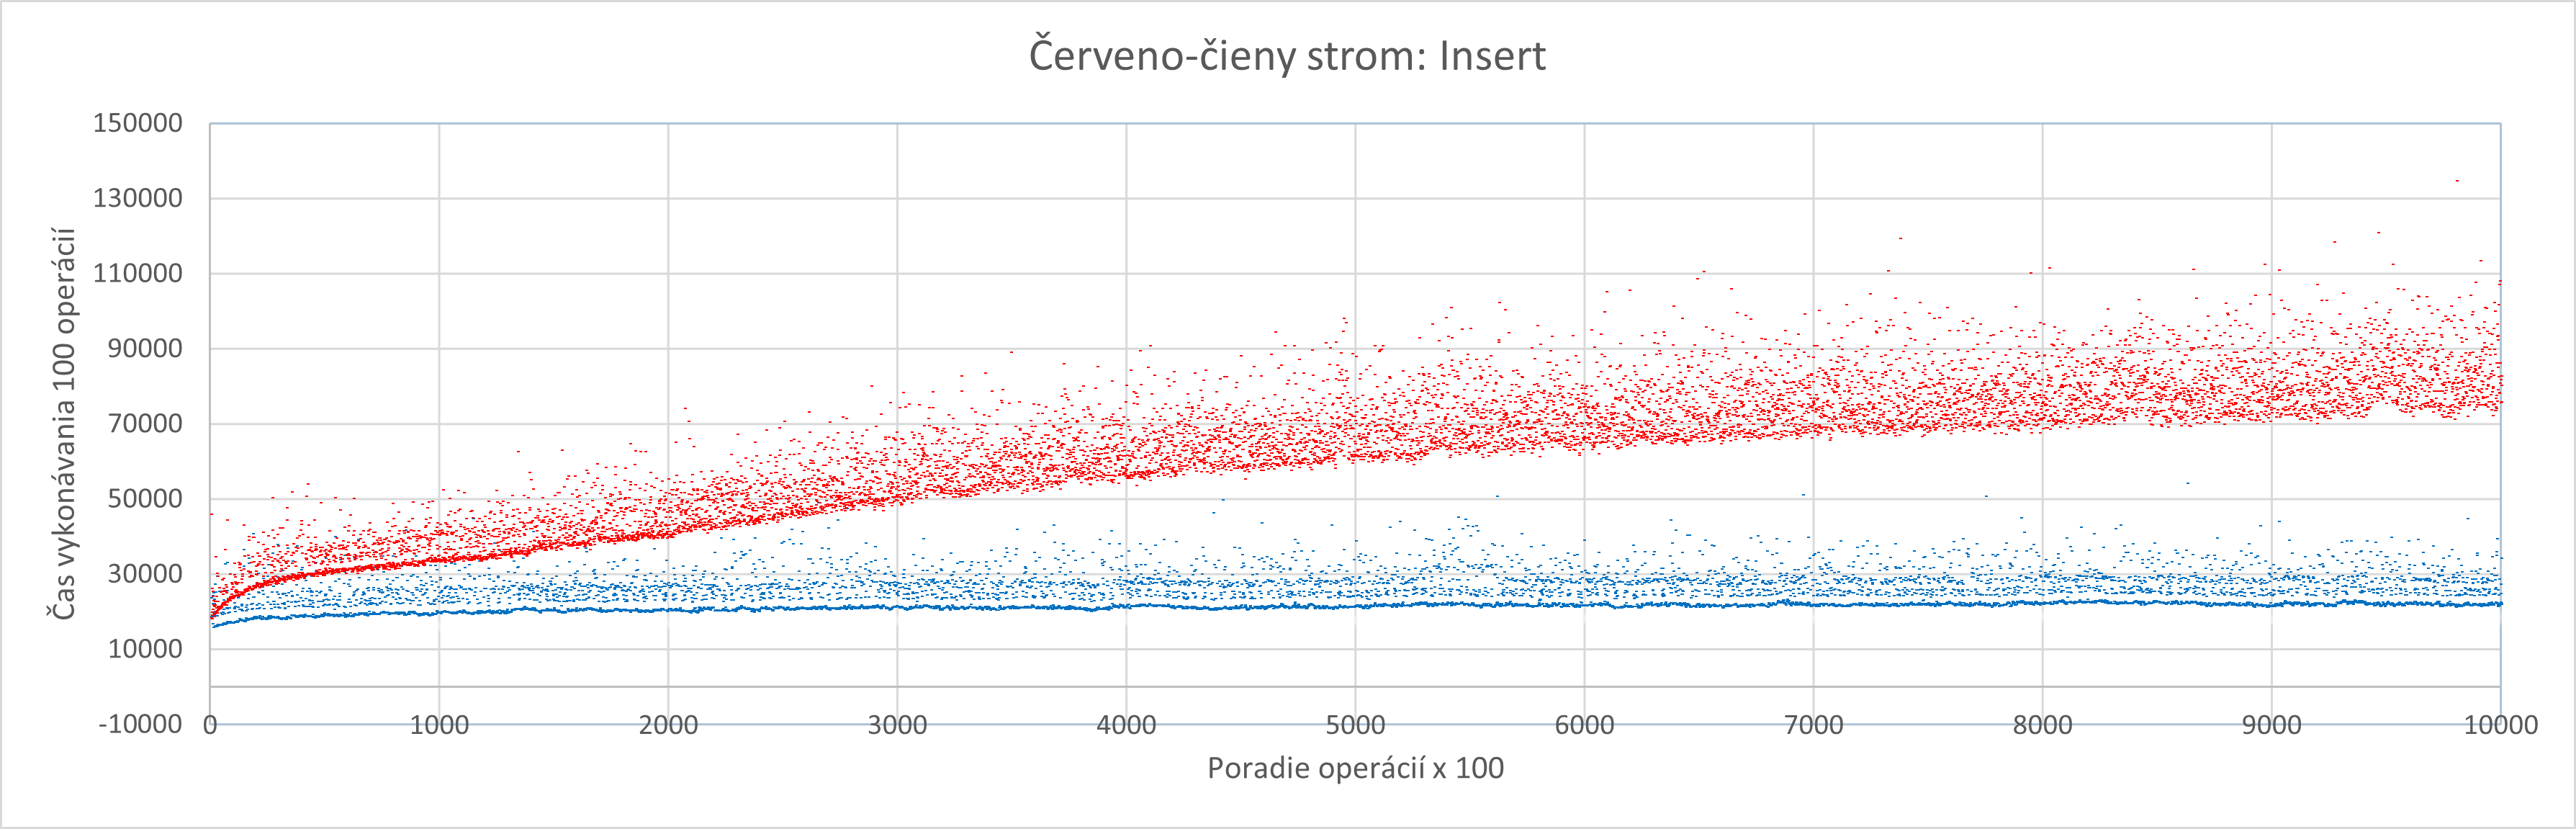
\includegraphics[width=\textwidth]{RB_Insert}
    \end{figure}
    \begin{figure}[!htbp]
        \centering
        \label{fig:figure2}
        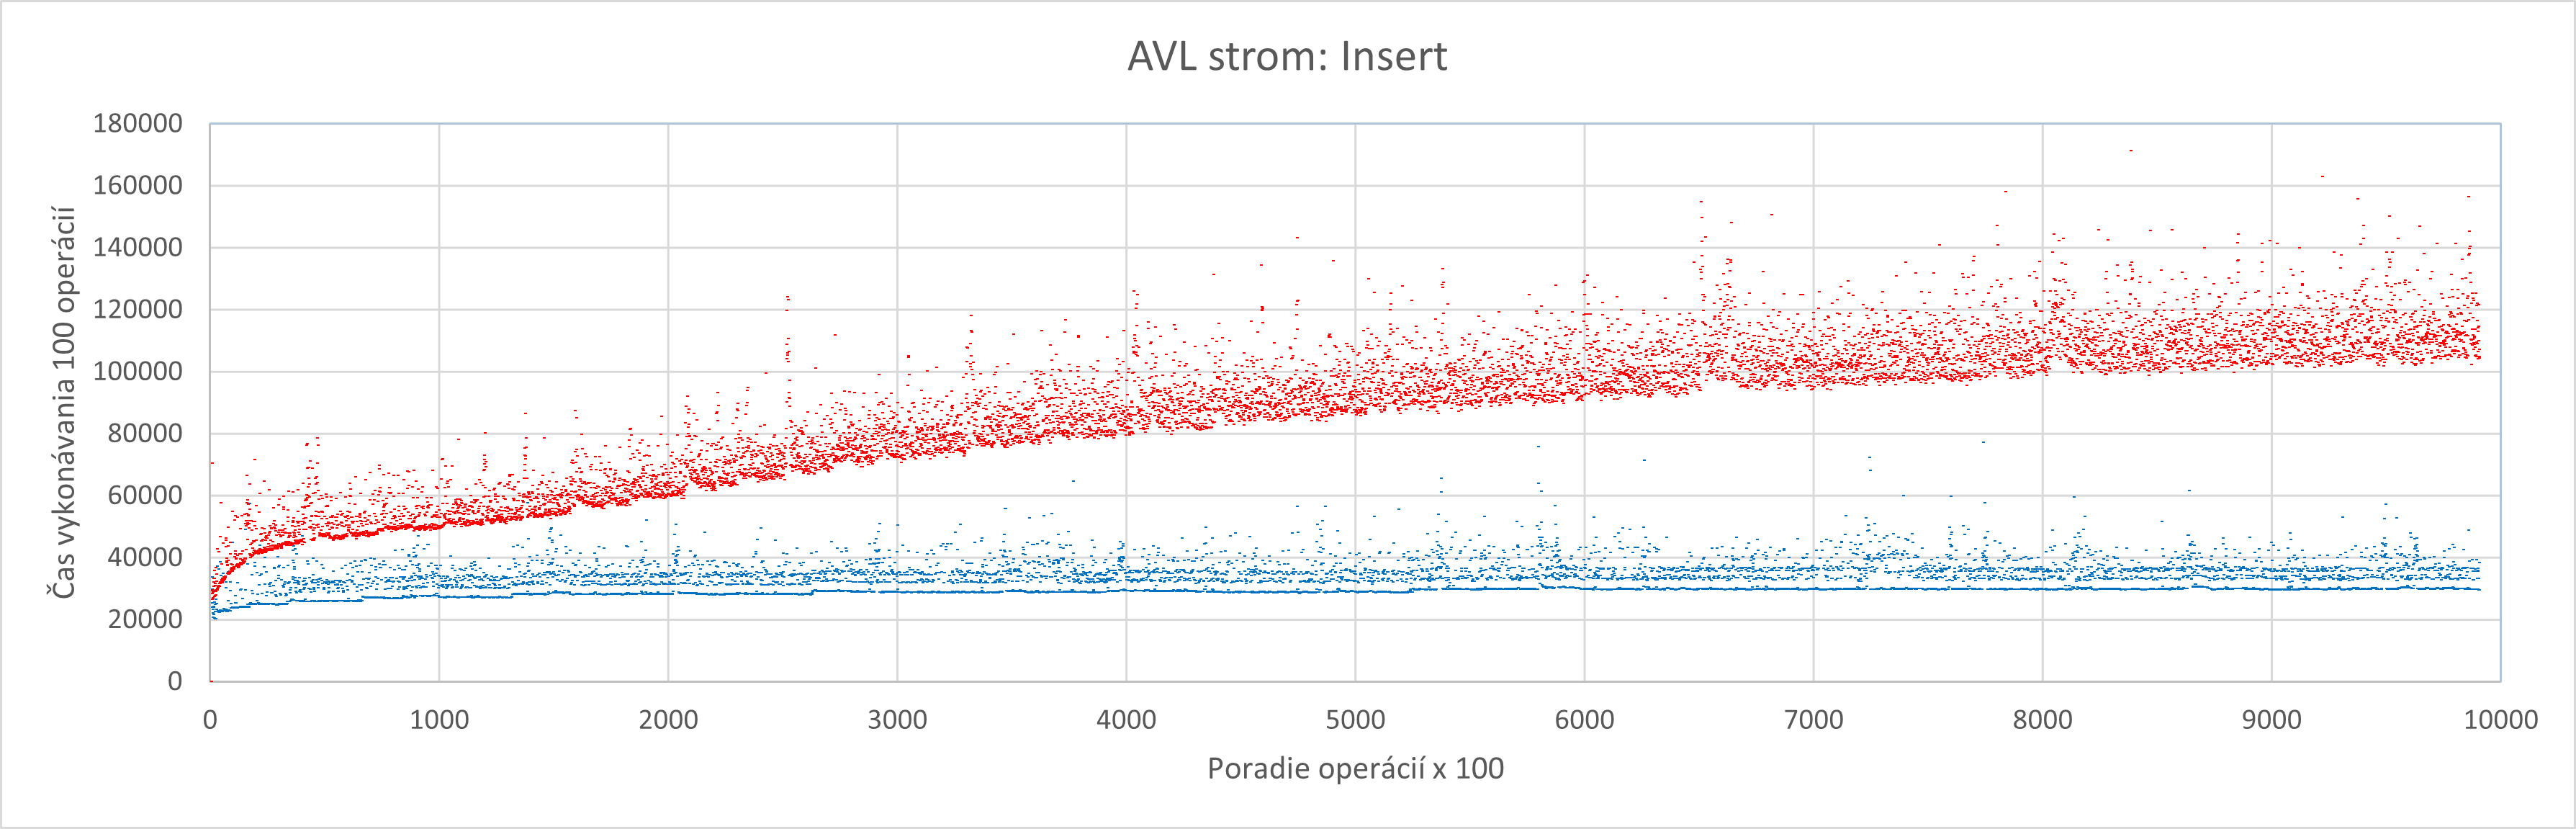
\includegraphics[width=\textwidth]{AVL_Insert}
    \end{figure}
    \begin{figure}[!htbp]
        \centering
        \label{fig:figure3}
        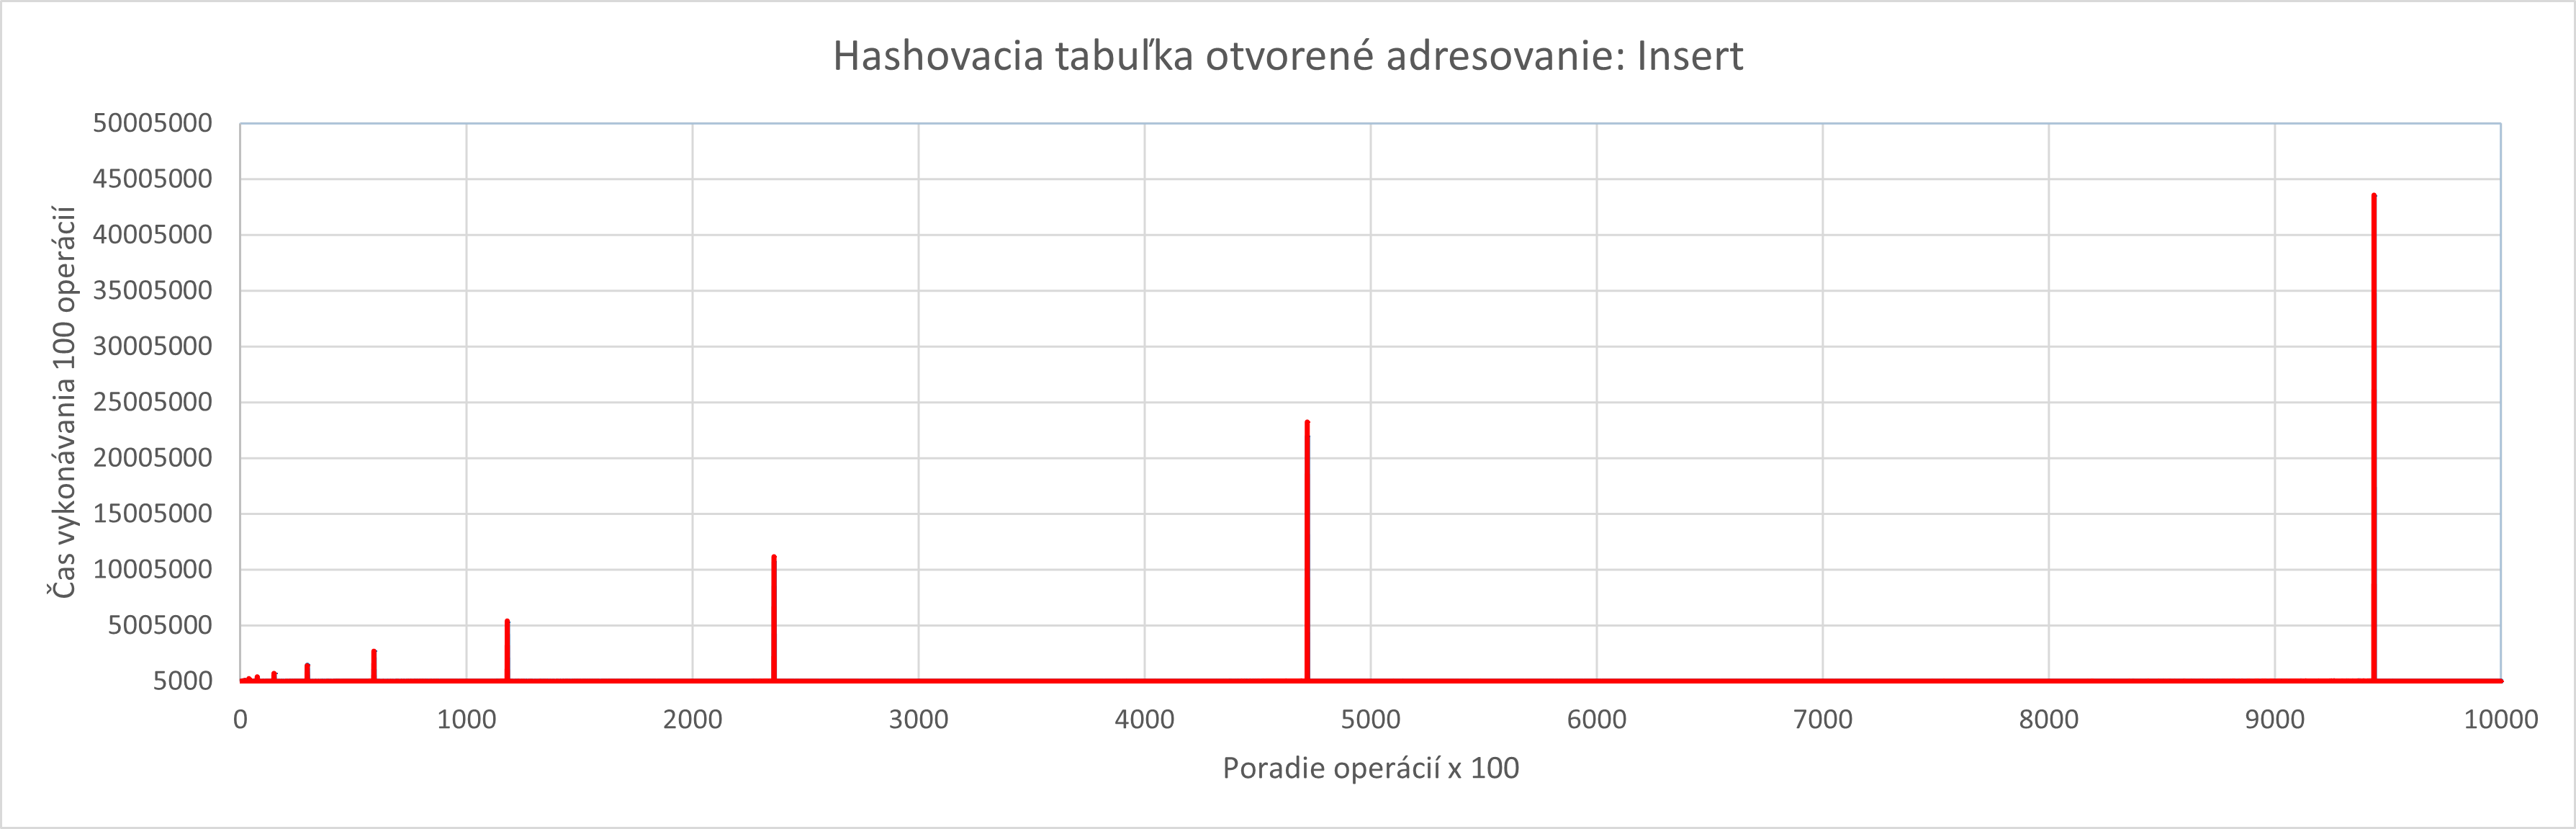
\includegraphics[width=\textwidth]{HashRobin_Insert}
    \end{figure}
    \begin{figure}[!htbp]
        \centering
        \label{fig:figure4}
        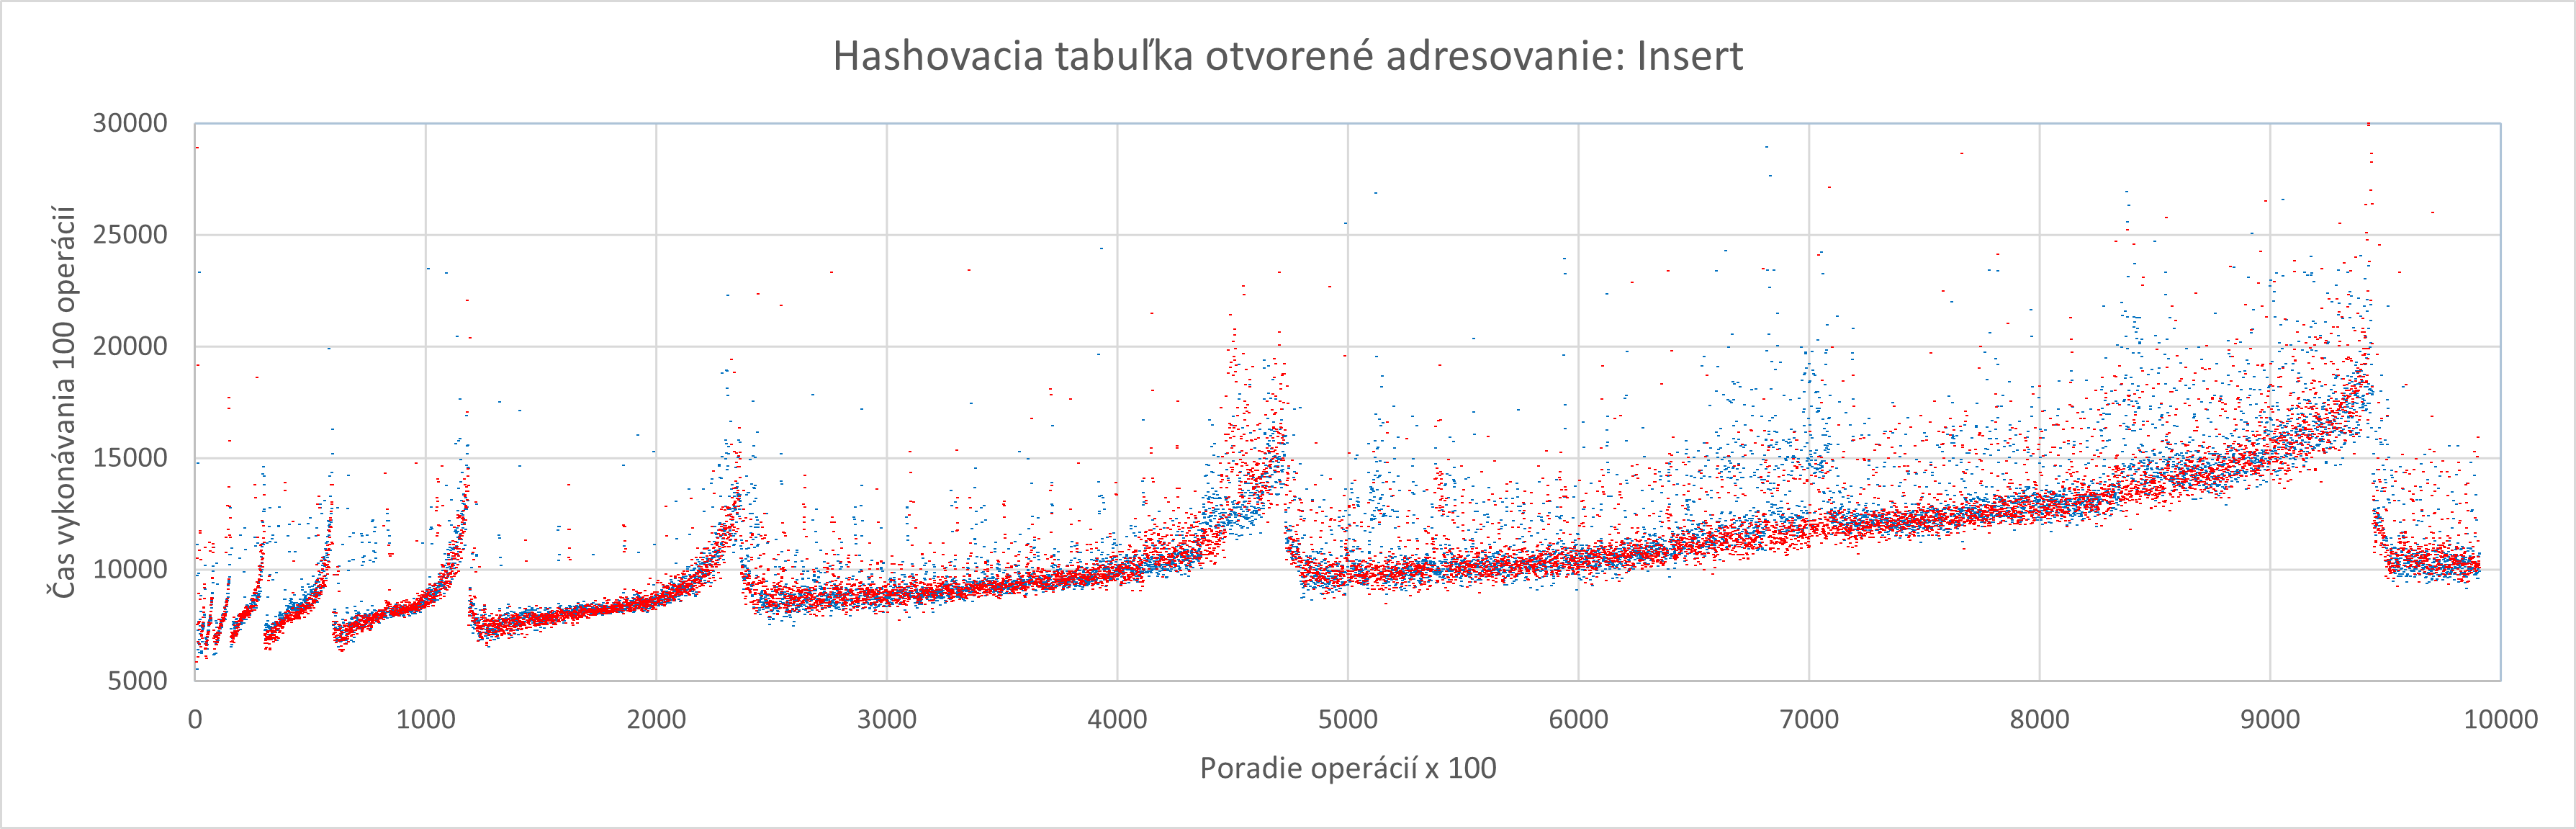
\includegraphics[width=\textwidth]{HashRobin_Insert_zoomed}
    \end{figure}
    \begin{figure}[!htbp]
        \centering
        \label{fig:figure5}
        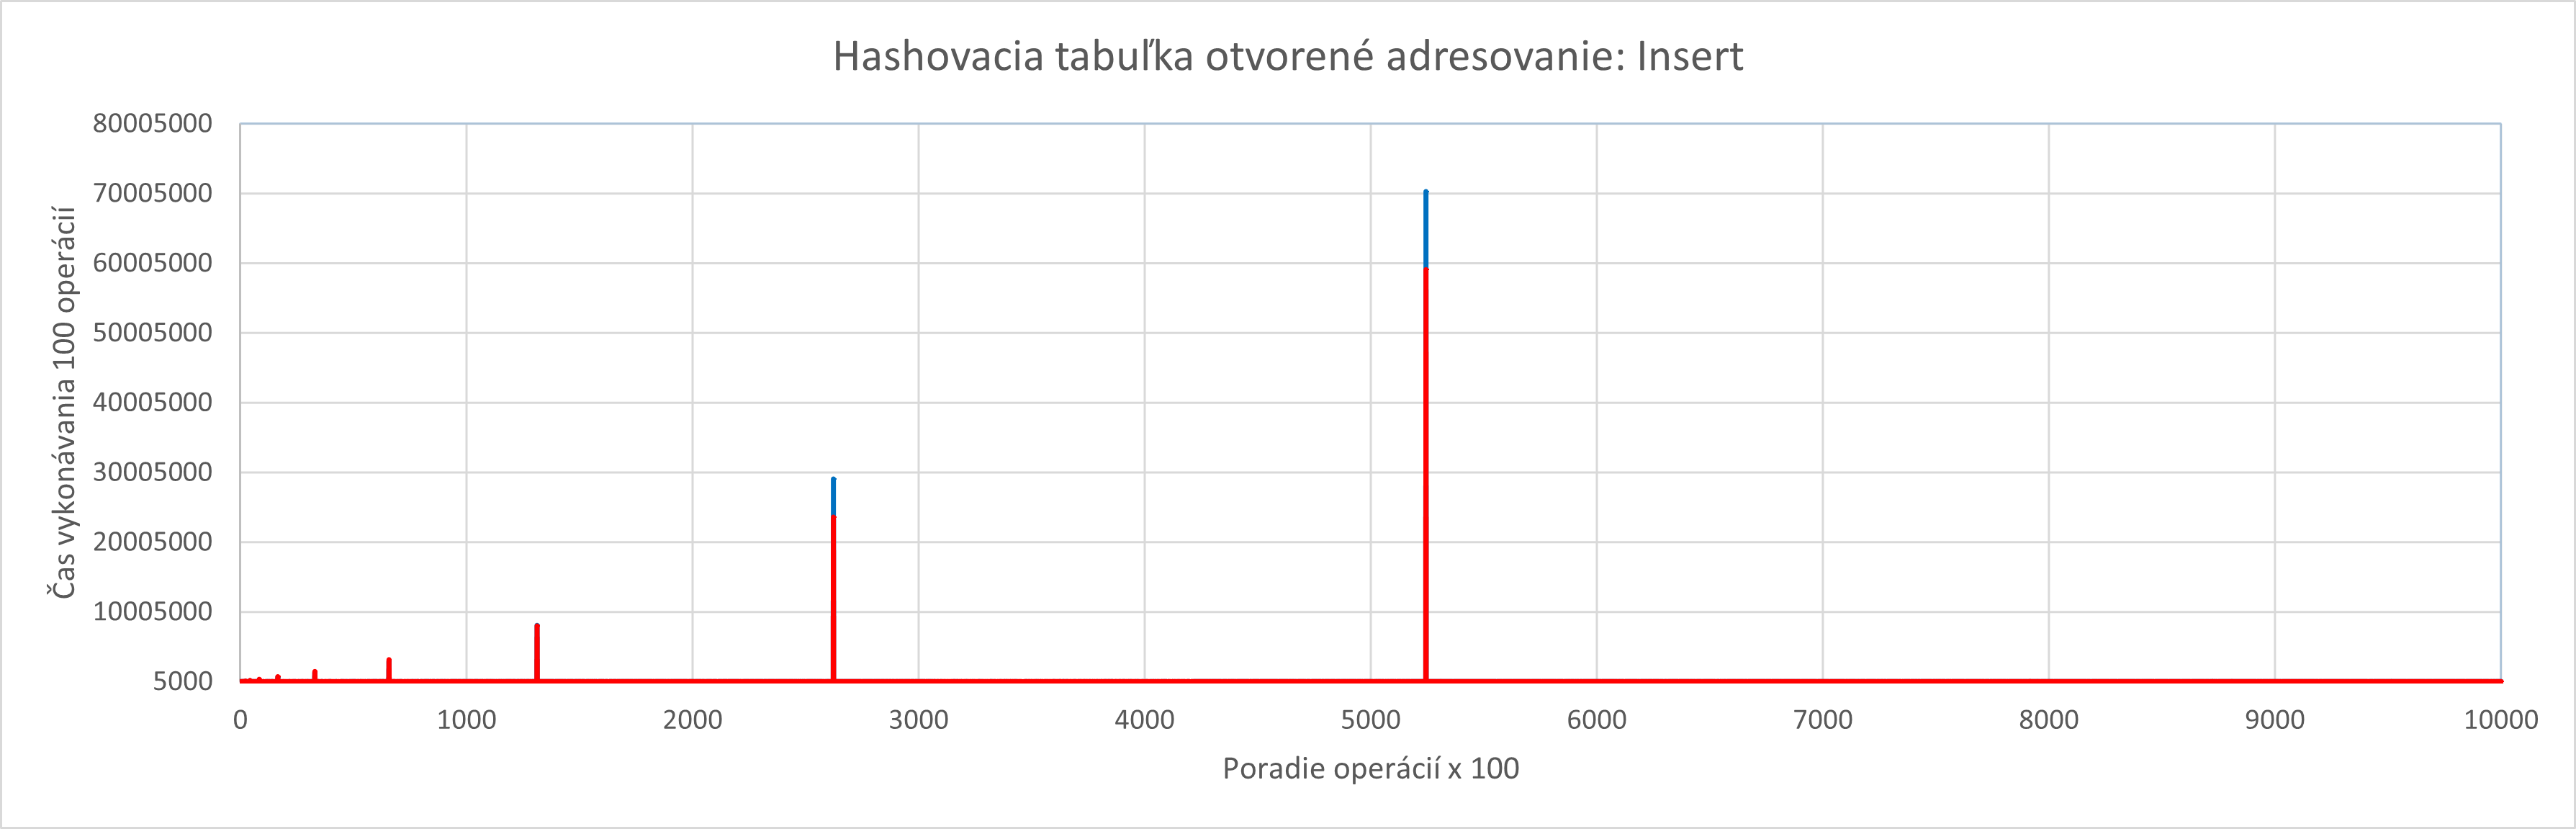
\includegraphics[width=\textwidth]{HashSC_Insert}
    \end{figure}
    \begin{figure}[!htbp]
        \centering
        \label{fig:figure6}
        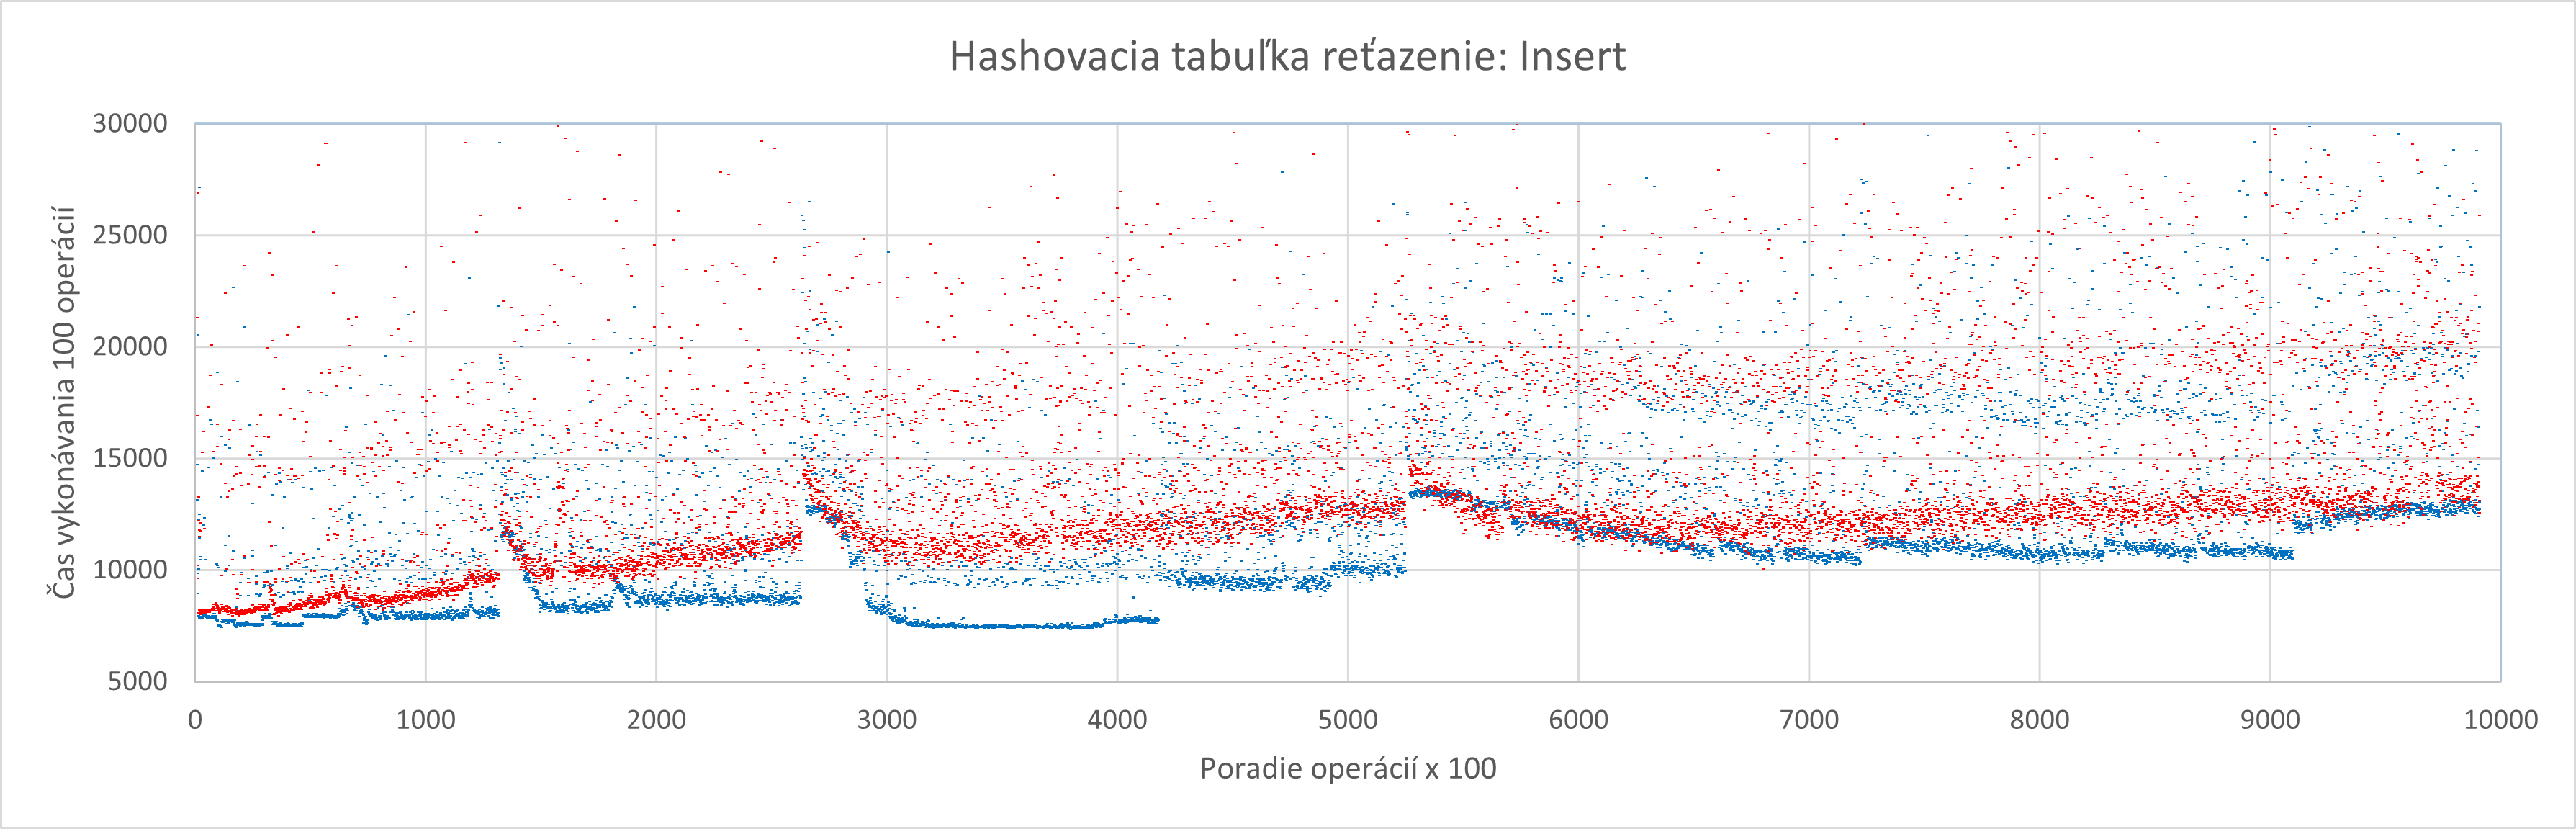
\includegraphics[width=\textwidth]{HashSC_Insert_zoomed}
    \end{figure}

    \FloatBarrier


    \newpage

    \includepdf[pages=-,offset= 0 -2cm, scale = .98,pagecommand=


    \section{Príloha A - Zadanie č.2 Vyhľadávanie v dynamických množinách}\label{sec:priloha-a-zadanie-c-2-vyhladavanie-v-dynamickych-mnozinach}]{DSA_zadanie2.pdf}

    \newpage


    \section{Príloha B – Upresnenie znenia zadania č. 2}\label{sec:priloha-b-upresnenie-znenia-zadania-c-2}
    \begin{itemize}
        \item {\makebox[8.5cm]{vlastná implementácia BVS\hfill}  – 02 body
            \begin{itemize}
                \item vyvažovanie
            \end{itemize}
            \item {\makebox[8.5cm]{vlastná implementácia hash tabuľky\hfill} – 02 body
                \begin{itemize}
                    \item riešenie kolízií
                    \item zväčšovanie tabuľky
                \end{itemize}
                \item {\makebox[8.5cm]{prevzatá implementácia BVS\hfill} – 01 bod
                \item {\makebox[8.5cm]{prevzatá implementácia hash tabuľky\hfill} – 01 bod
                \item  {\makebox[8.5cm]{testovací program\hfill} – 02 body
                    \begin{itemize}
                        \item vytvoriť BVS/hash o veľkosti počtu prvkov 1 000/25 000/100 000
                        \item používajte rovnaké prvky pre BVS aj has tabuľku
                        \item operácia insert - čas potrebný na:
                        \begin{itemize}
                            \item vytvorenie
                            \item 1 prvok
                            \item 25 \% prvkov
                            \item zopakujte 5 krát
                        \end{itemize}
                        \item operácia search - čas potrebný na:
                        \begin{itemize}
                            \item 1 prvok
                            \item 5 \% prvkov
                            \item zopakujte 5 krát
                        \end{itemize}
                    \end{itemize}
                    \item {\makebox[8.5cm]{dokumentácia\hfill}                    – 02 body
                        \begin{itemize}
                            \item opisy algoritmov
                            \item spôsob testovania
                            \item dosiahnuté výsledky
                        \end{itemize}
                        \item {\makebox[8.5cm]{celkom:\hfill}    – 10 bodov
    \end{itemize}


\end{document}